\section{Results}
\label{SECIV}\label{sec:results}

\begin{figure}
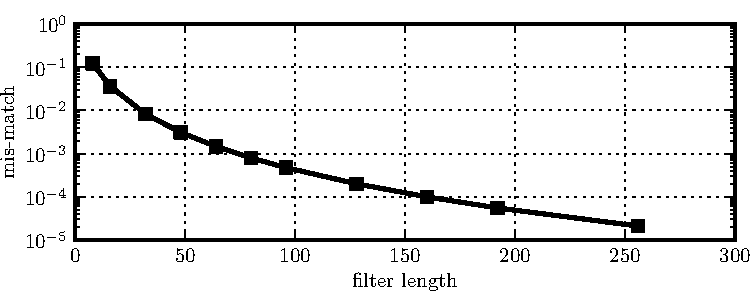
\includegraphics{resamp_mm.pdf}
\caption{\label{fig:resamp_mm}}
\end{figure}



\FIXME{
I would like to see this section changed to emphasize the low-latency time domain filtering
1. Use a live simulated white noise source (this ignores the latency of whitening, but that goes
beyond the scope of this paper, and we mention this and perhaps suggest some exporation
2. Use TD filtering of N templates
3. Present the performance and latency and provide estimates for number of cores required for realtime ALIGO search based on current infrastructure
4. Compute the impulse responses of the templates and histogram the SNR loss for the SVD and time/slice/resampling
5. Put  a tee after some of the low frequency stages and perhaps test the possibility of
predictive filtering (also with latency measurments)
This will remove the complications of running a full pipeline.  We need to sort things out before
we do that, and this paper should not be delayed any further.  The above tests will make the point we need to make
}

\subsection{Detector noise characteristics}

We tested the new detection method with mock Advanced \textsc{ligo} data having a power spectrum prescribed by the ``zero detuning, high power'' noise model in \cite{Shoemaker:2009p9770}.
